% This is a simple sample document.  For more complicated documents take a look in the exercise tab. Note that everything that comes after a % symbol is treated as comment and ignored when the code is compiled.

\documentclass{article} % \documentclass{} is the first command in any LaTeX code.  It is used to define what kind of document you are creating such as an article or a book, and begins the document preamble

\usepackage{amsmath} % \usepackage is a command that allows you to add functionality to your LaTeX code

\usepackage[T1]{fontenc}
\usepackage{titling}
\usepackage{graphicx}
\graphicspath{ {./images/} }
\newtheorem{proof}{Proof}

\setlength{\droptitle}{-10em}   % This is your set screw

\title{Discrete Mathematics Question Set 1}
\author{Abrar Habib}

% The preamble ends with the command \begin{document}
\begin{document} % All begin commands must be paired with an end command somewhere
    \maketitle % creates title using information in preamble (title, author, date)
    
    \textbf{1.} Simplify the statements so that no negation is outside a quantifier or an expression involving logical
    connectives. (20 pt.)

    \paragraph*{a.}
    $\neg \forall x \forall y(P(x,y) \lor Q(x,y))$

    $$\neg \forall x \forall y (P(x,y)\lor Q(x,y))$$
    We can change the universal quantifier to the existential quantifier because $\neg \forall = \exists$ and factor the $\neg$ into the $\land$ operation.
    The equation now becomes:
    $$\exists x \forall y \neg(P(x,y)\lor Q(x,y))$$
    Apply DeMorgans Law:
    $$\exists x \forall y (\neg P(x,y) \land \neg Q(x,y))$$
    We cannot simplify any more.
    \paragraph*{b.}
    $\neg (\exists x \exists y \neg P(x,y)\land \forall x \forall y Q(x,y))$
    Distribute the outer negation and using DeMorgans Law:
    $$\neg \exists x \neg \exists y \neg\neg P(x,y) \lor \neg\forall x \neg\forall y \neg Q(x,y)$$
    Simplify statements:
    $$\forall x \forall y P(x,y) \lor \exists x \exists y \neg Q(x,y)$$
    We cannot simplify any more.

    \newpage
    \textbf{2.} Prove the validity of this argument:

    Premises:

    \begin{align}
        (p \land t) \rightarrow (r \lor s) &\\
        q \rightarrow (u \land t) &\\
        u \rightarrow p &\\
        \neg s
    \end{align}

    Conclusion:
    $$q \rightarrow r$$
    
    % 1) & $\neg s$                        & Premise \\ 
    % 2) & $(p\wedge t)\implies (r\vee s)$ & Premise \\  
    % 3) & $(p\wedge t)\implies r$         & 1, 2 Disjunctive Syllogism



    \begin{tabular}{ l l l }
        1) & $(p \land t) \rightarrow (r \lor s)$ & Premise \\

        2) & $(p \land t)$                        & Premise \\

        3) & $p$                                  & 2, Specification \\

        4) & $t$                                  & 2, Specification \\

        5) & $q$                                  & Premise \\

        6) & $q \rightarrow ( u \land t)$         & Premise \\

        7) & $u \land t$                          & 5,6 Modus Ponens \\

        8) & $u \rightarrow p$                    & Premise \\

        9) & $u \rightarrow (p \land t)$          & 3, 4 Conjunction \\ 

        10) & $(p \land t) \rightarrow (r \lor s)$ & Premise \\ 

        11) & $u \rightarrow (r \lor s)$           & 9, 10 Hypothetical Syllogism \\ 

        12) & $\neg s$                             & Premise \\  

        13) & $u \rightarrow r$                   & 11, 12 Disjunctive Syllogism \\ 

        14) & $(u \land t) \rightarrow r$         & 7, 13 Conjunction \\

        15) & $q \rightarrow (u \land t)$         & Premise \\ 

        16) & $q \rightarrow r$                   & 14, 15 Hypothetical Syllogism \\       
    \end{tabular}
    \\\\
    Other Method:

    \begin{tabular}{ l l l }
        1) & $q$ & Premise \\

        2) & $q \rightarrow (u \land t)$  & Premise \\

        3) & $u \land t$            & 1,2 Modues Ponens \\

        4) & $u$                & 3, Specification \\

        5) & $t$                 & 3, Specification \\

        6) & $u \rightarrow p$         & Premise \\

        7) & $p$              & 4, 6 Modus Ponens \\

        8) & $p \land t$       & 5, 7 Specification \\

        9) & $(p \land t) \rightarrow (r \lor s)$    & Premise \\ 

        10) & $(r \lor s)$ & 8,9 Modus Ponens \\ 

        11) & $\neg s$           & Premise \\ 

        12) & $r$              & 10, 11 Disjunctive Syllogism \\ 
        
        13) & $q \rightarrow r$ & 1,12 Conditional Proof \\
    \end{tabular}

    Because $q$ is implied as a premise, and we have derived $r$ using rules of 
    
    inference, we can use conditional proof as a method of saying $q \rightarrow r$.   


    \newpage

    \textbf{3.} Is this statement a tautology? (Explain using a truth table) (10 pts.)
    
    $$(\neg q \land (p \rightarrow q)) \rightarrow \neg p$$

    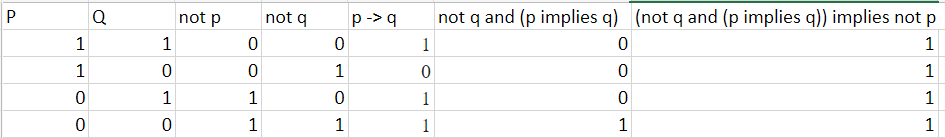
\includegraphics[scale=0.9]{figure1.png}

    This statement is a tautology.
    
    \newpage

    \textbf{4.} Prove that if n is an integer and $n^3 + 5$ is odd, then n is even using (20 pts.)
    
    a) proof by contraposition

    b) proof by contradiction

    \begin{proof}
        Assume n is an odd integer.
    
        So $n = 2k+1$ for some integer k.
    
        Plugging in $n = 2k+1$ into $n^3+5$ we get 
        \begin{equation*}
            \begin{aligned}
                (2k+1)^3+5 &\\
                8k^3+12k^2+6k+1+5 &\\
                8k^3+12k^2+6k+6
            \end{aligned}
        \end{equation*}
        
        We can factor out a 2 from this equation to get $$2(4k^3+6k^2+3k+3)$$
        
        Since k was an integer, $8k^3+12k^2+6k+6$ is also an integer.

        Because we assumed n was odd and $n^3+5$ can be represented as $2(j)$ where 
        
        $j = 4k^3+6k^2+3k+3$, 
        
        n has to be even.

    \end{proof}

    \begin{proof}
        Suppose that if n is an integer and $n^3+5$ is even, then n has to 
        
        be odd.

        If n is odd, it can be represented as $2k+1$ for some integer k.
        
        We can plug it into $n^3+5$ 
        \begin{equation*}
            \begin{aligned}
                (2k+1)^3+5 &\\
                8k^3+12k^2+6k+1+5 &\\
                8k^3+12k^2+6k+6 &\\
                2(4k^3+6k^2+3k+3)
            \end{aligned}
        \end{equation*}

        Since we assumed that n was an integer, $2(4k^3+6k^2+3k+3)$ must also be 
        
        an integer.

        Because $n^3+5$ can be represented as $2(j)$ where $j = (4k^3+6k^2+3k+3)$,
        
        this directly contradicts with our claim that n has to be odd. 

        Therefore, n is even.
    \end{proof}


    \newpage

    \paragraph*{5.}
    Determine whether each of these statements is true or false and explain the reason briefly. (30 pts.)

    a) $x \in \left\lbrace x \right\rbrace$

    This is true. The set $\left\lbrace x \right\rbrace$ contains one element which is $x$.

    b) $\left\lbrace x \right\rbrace \subseteq \left\lbrace x \right\rbrace$

    This is true. Every element in $\left\lbrace x \right\rbrace$ is part of the set $\left\lbrace x \right\rbrace$. 
    
    c) $\left\lbrace x \right\rbrace \in \left\lbrace x \right\rbrace$
    
    This is false. The set $\left\lbrace x \right\rbrace$ does not have within itself another set, only an 
    
    element $x$.

    \newpage

    \paragraph*{6}  Let A, B, and C be sets. Using membership or Venn diagram show that
    \\\\
    a) $(A \cup B) \subseteq (A \cup B \cup C)$

    $A \cup B \cup C$ is a union of all three sets such that it contains 
    
    all elements of all three sets. 

    Therefore, the elements of $A \cup B$ are part of the union of all three sets.

    Therefore, $A \cup B \subseteq (A \cup B \cup C)$ is true.
    \\\\
    b) $(A - B) - C \subseteq A-C$

    $(A-B) - C$ is the set of all elements that are unique to only A. 

    The set $A - C$ is the set of all elements that are unique to A, but also includes 
    
    elements from B as well. 

    Therefore, the elements in $(A - B) - C$ which only includes elements 
    
    unique to A is a subset of $A - C$ which includes all elements unique to 
    
    set A, plus elements of set B.


    \end{document} % This is the end of the document